
A proposta deste trabalho envolve a união dos cinco cursos de engenharia presentes no campus UnB - Gama, com o objetivo de solucionar os problemas apresentados acima. A proposta inicial de solução se baseia no desenvolvimento de um aspirados de pó autônomo, com capacidade de regarga de bateria automaticamente. A implementação desta proposta envolve diversas áreas de conhecimento e estará melhor detalhada nas seções seguintes.

A organização da apresentação da solução está baseada em sub-sistemas que integrados resultarão na solução como um todo. 

\section{Requisitos do sistema} % (fold)
\label{sub:requisitos_do_sistema}

Os requisitos do sistema estão apresentados na tabela \ref{tab:requisitos}.

\begin{table}[H]
\centering
\caption{Requisitos do sistema}
\label{tab:requisitos}
\begin{tabular}{|c|c|}
\hline
\rowcolor[HTML]{C0C0C0} 
\textit{\textbf{Requisitos Gerais}}                                                                 & \textit{\textbf{Requisitos Específicos}}            \\ \hline
                                                                                                    & Aspirar o pó                                        \\ \cline{2-2} 
                                                                                                    & Se locomover pelo ambiente                          \\ \cline{2-2} 
                                                                                                    & Responder a obstáculos no ambiente                  \\ \cline{2-2} 
\multirow{-4}{*}{Limpar um cômodo}                                                                  & Se comunicar com a central de processamento         \\ \hline
                                                                                                    & Retornar a base                                     \\ \cline{2-2} 
                                                                                                    & Gerenciar status da bateria                         \\ \cline{2-2} 
\multirow{-3}{*}{Se recarregar sozinho}                                                             & Recarregar a bateria                                \\ \hline
                                                                                                    & Possuir sistema de acompanhamento do status do robô \\ \cline{2-2} 
                                                                                                    & Possuir sistema de agendamento de limpeza           \\ \cline{2-2} 
                                                                                                    & Possuir sistema de start/stop                       \\ \cline{2-2} 
\multirow{-4}{*}{\begin{tabular}[c]{@{}c@{}}Possuir sistema de controle\\ a distância\end{tabular}} & Gerar relatório de atividades                       \\ \hline
\end{tabular}
\end{table}
% section requisitos_do_sistema (end)
\section{Alimentação} % (fold)
\label{sub:alimentação}
	A equipe de engenharia de energia tem como meta desenvolver o sistema de alimentação para o funcionamento do robô aspirador. Existem diversas possibilidades de fornecer a energia necessária pra suprir a potência requerida pelo sistema, sendo que a mais usual seria a utilização de baterias, que podem ser sintetizadas como um conjunto de pilhas responsável por transformar energia química em energia elétrica, por meio de duas placas de composição diferente, chamadas eletrodos, sendo sempre um positivo e um negativo. 

	A fonte de alimentação ideal para o sistema segue alguns requisitos essenciais, como ter autonomia mínima de 30 minutos (tempo suficiente para aspirar um cômodo). Alguns parâmetros como tensão e corrente ainda não podem ser definidos nesta etapa do projeto. Buscando as alternativas disponíveis dentro desse universo nos deparamos com a opção das baterias NIMH, que apresenta uma gama com alguns modelos disponíveis e com valores variáves de tensão e corrente.
	
	A recarga dessas baterias varia de acordo com a potência fornecida por cada uma, no entanto alguns fabricantes produzem carregadores que retiram a tensão alternada de 220v, 60Hz para a tensão contínua da bateria escolhida. O manual do carregador informa o tempo máximo de recarga de 45 minutos para o modelo mais potente de bateria, número esse que pode ser de apenas 15 minutos em alguns casos. Dentre as opções disponíveis, estão dispostas três nas imagens abaixo (18v, 14.4v e 12.4v/ 3,3Ah e 2,6Ah).

	\begin{figure}[H]
		\centering
		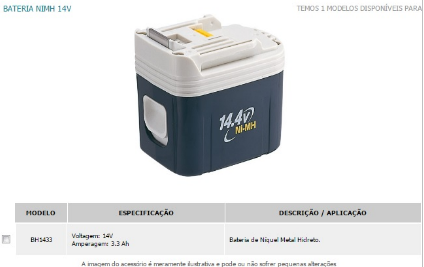
\includegraphics[scale=0.55]{figuras/bateria_1.png}
		\caption{Bateria de 14.4v.}
		\label{img:bateria_1}
	\end{figure}

	\begin{figure}[H]
		\centering
		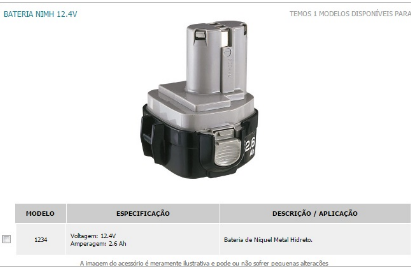
\includegraphics[scale=0.55]{figuras/bateria_2.png}
		\caption{Bateria de 12.4v.}
		\label{img:bateria_2}
	\end{figure}
	
	\begin{figure}[H]
		\centering
		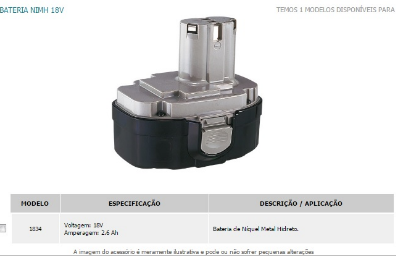
\includegraphics[scale=0.55]{figuras/bateria_3.png}
		\caption{Bateria de 18v.}
		\label{img:bateria_3}
	\end{figure}

	Uma outra alternativa para suprir a alimentação do aspirador seria o uso de supercapacitores. Tal opção oferece um valor consideravelmente maior de ciclos de carga (10 000 contra 400-6000), além um tempo de recarga muito reduzido se comparado com as baterias. Entre os fatores desfavoráveis pode-se citar a fragilidade, que acarreta em um maior cuidado no manuseio, o elevado custo de mercado além  da falta de informações técnicas obtidas até o momento.
% section alimentação (end)

\section{Navegação} % (fold)
\label{sub:automação}
	A solução referente à navegação possui enfoque principal no algoritmo de controle que trabalhará a trajetória a ser percorrida, a identificação de obstáculos e replanejamento da trajetória e a lógica de controle para retorno à base. Diversas possibilidades foram estudadas e analisadas, desde o planejamento de rota partindo com formato espiral, até trajetórias aleatórias com simples desvios de obstáculos.

	A partir e comparações e estudo de concorrentes, como o robô \textit{Roomba}\footnote{https://www.irobot.com.br/}, por exemplo, observou-se que na grande maioria, o sistema de navegação escolhido pelos fabricantes é baseado em trajetórias aleatórias. Segundo \cite{robo_limpeza_domesti}, a utilização de navegação aleatória garante um bom desempenho, já que com o passar do tempo, o robô consegue acessar o cômodo como um todo. Dessa forma, optou-se pela utilização de um algoritmo de navegação baseado em trajetória aleatória para o desenvolvimento do sistema \textit{R2-PI2}.

	Um dos grandes problemas encontrados na navegação é referente a volta à base por parte do robô. Identificar onde a base se encontra e traçar uma rota até a mesma é uma tarefa que necessita de algumas ferramentas, como a utilização de sinais e sensores para comunicação entre a base e o robô. Para isso, optou-se pela utilização de 3 (três) sensores infra-vermelho emitidos pela base com uma angulação de 45º entre eles, fazendo com que o robô possa identificar o sinal e navegar até sua fonte, a base.
% section automação (end)

\section{Estrutura e Locomoção do robô} % (fold)
\label{sub:locomocao}
	
	O robô, de forma autônoma, deve percorrer todo o cômodo escolhido para limpá-lo para isso deve ser desenvolvido todo o sistema de locomoção dele, incluindo as rodas, motor, caixa de redução e todo o estudo dinâmico relacionado. Foram cogitadas duas soluções para a estrutura do robô e sua forma de locomoção, de forma que a segunda solução foi escolhida. A escolha da segunda solução se justifica com base nos requisitos do sistema de sensoriamento quanto a posição de sensores pela estrutura e devido ao maior erro propagado pela primeira solução na navegação inercial do sistema. 

	\subsection{Solução 1} % (fold)
	\label{sub:solução_1}

		O robô seria composto de uma chapa retangular de alumínio de 400mm x 300mm x 5mm, que servirá como base para a distribuição e união dos componentes do projeto. Essa base retangular poderá ser usinada para outra forma caso haja necessidade de diminuição do tamanho do robô. O material escolhido para a base foi o alumínio pela sua leveza, resistência e preço. Sua área  de superfície é capaz de abrigar todos os componentes do aspirador e ainda possui espaços para criar novas soluções ou até mesmo de componentes para a refrigeração dos subsistemas do robô.

		O sistema de tração dessa base será feito por uma esteira tipo lagarta, muito utilizada em tanques de guerra. Esse sistema é bastante robusto e aguentaria o peso de todo a estrutura sem problemas. Isso tiraria a necessidade de colocar um sistema de suspensão.

		A estrutura do aspirador e seus componentes:

		\begin{itemize}
			\item 2 motores com caixa de redução ligados a chapa de alumínio;
			\item Os eixos que ligaram as rodas a chapa de alumínio serão feitos com aço e serão usinados nas pontas para fazer roscas que irão fixar as rodas;
			\item 4 engrenagens grandes que serão utilizadas como rodas;
			\item 2 engrenagens menores que irão ser ligadas direto nos dois motores;
			\item Conectores múltiplos, do tipo que se usa em chuveiros para ligar os eixos na chapa de alumínio;
			\item Correntes de bicicleta que ligaram as engrenagens e farão o papel de esteira.
		\end{itemize}

		Entre esses dois sistemas foi escolhido o segundo pela sua construção ser mais robusta e suporta mais os esforços que será submetido o robô. Um grande problema do primeiro sistema é que a sustentação da estrutura se daria no próprio eixo do motor, que é de plastico, o que poderia causar a quebra do sistema, já no segundo sistema a sustentação é feita nos eixos, que são feitos de aço.
		
		\begin{figure}[H]
			\centering
			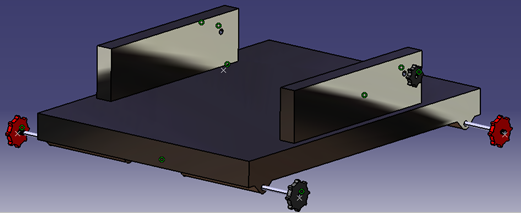
\includegraphics[scale=0.8]{figuras/rascunho_estrutura.png}
			\caption{Rascunho da estrutura - Solução 1}
			\label{img:rascunho1}
		\end{figure}


		\subsection{Solução 2} % (fold)
		\label{sub:solução_2}
			
			O robô aspirador terá forma circular. Esse formato foi escolhido para facilitar as manobras de curvas, aumentando a área que ele irá percorrer. Outra vantagem que esse formato fornece é a questão do controle autônomo dele, assim facilita a distribuição dos sensores e o próprio controle do movimento do robô, pois resulta em menos erros. A estrutura do robô deve ser tal para suportar as cargas dos equipamentos do interior do robô como os sensores, motores, coolers e o sistema de sucção sem que sofra deformações. Além dessas forças deve-se também ser resistente à fadiga, já que estará sujeito a cargas contínuas e repetidas, e a impactos contra objetos ou paredes. Um material que já é utilizado em muitas aplicações pois apresenta boa propriedades é o Alumínio. A tabela a seguir mostra alguns valores das propriedades mecânicas do alumínio.


			ARRUMAR TABELA!!!!!
			\begin{figure}[H]
				\centering
				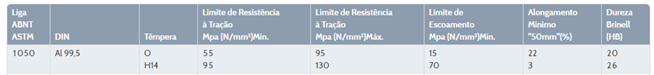
\includegraphics[scale=0.8]{figuras/tabela_estru1.png}
				\caption{Propriedades mecânicas do alumínio. Adaptado de \href{http://www.shockmetais.com.br/especificacoes/aluminio/pmec}{Shockmetais}}
				\label{img:rascunho1}
			\end{figure}

			Então será construída uma base circular de alumínio de 40 cm de diâmetro.

        	Com relação a movimentação do robô 3 rodas serão suficientes para garantir o equilíbrio. Duas rodas serão tracionadas uma livre.  A roda livre é do tipo esfera e as outras duas serão de um kit motor redução, que junto à roda está montado o motor com uma caixa de redução para aumentar o torque. A mudança de direção e giro do robô é realizada alternando a potência fornecida em cada roda ou invertendo o sentido de rotação, por exemplo para fazer com que ele gire para a esquerda, deve diminuir a potência da roda esquerda e manter a potência da roda direita. As figuras seguintes ilustram as rodas e motores utilizados.

        	\begin{figure}[H]
				\centering
				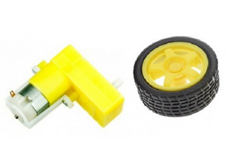
\includegraphics[scale=0.7]{figuras/motor_roda.png}
				\caption{Kit motor redução.}
				\label{img:kit_motor}
			\end{figure}

			\begin{figure}[H]
				\centering
				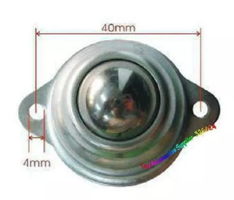
\includegraphics[scale=0.7]{figuras/esfera.png}
				\caption{Roda do tipo esfera.}
				\label{img:esfera}
			\end{figure}

			As especificações da roda e do motor são mostradas na tabela \ref{tab:motor_red}:

			\begin{table}[H]
				\centering
				\caption{Especificação motor de redução}
				\label{tab:motor_red}
				\begin{tabular}{|c|c|}
					\hline
					\multicolumn{2}{|c|}{\cellcolor[HTML]{C0C0C0}\textbf{Especificação Motor}} \\ \hline
					\textit{\textbf{Tamanho}}                            & 69x37x22,7mm        \\ \hline
					\textit{\textbf{Peso}}                               & 29g                 \\ \hline
					\textit{\textbf{Formato}}                            & 90 graus            \\ \hline
					\textit{\textbf{Tensão de operação}}                 & 3 a 6V              \\ \hline
					\textit{\textbf{Relação de transmissão}}             & 1:120               \\ \hline
					\textit{\textbf{Velocidade a 3V(sem carga)}}         & 100 rpm             \\ \hline
					\textit{\textbf{Corrente a 3V(sem carga)}}           & 60 mA               \\ \hline
					\textit{\textbf{Corrente a 3V(com carga)}}           & 260 mA              \\ \hline
					\textit{\textbf{Torque a 3V}}                        & 1.20 kgf-cm         \\ \hline
					\textit{\textbf{Velocidade a 6V(sem carga)}}         & 200 rpm             \\ \hline
					\textit{\textbf{Corrente a 6V(sem carga)}}           & 71 mA               \\ \hline
					\textit{\textbf{Corrente a 6V(com carga)}}           & 470 mA              \\ \hline
					\textit{\textbf{Torque a 6V}}                        & 1.92 kgf-cm         \\ \hline
					\textit{\textbf{Diâmetro externo do eixo}}           & 5,4 mm "I"          \\ \hline
				\end{tabular}
			\end{table}

			\begin{figure}[H]
				\centering
				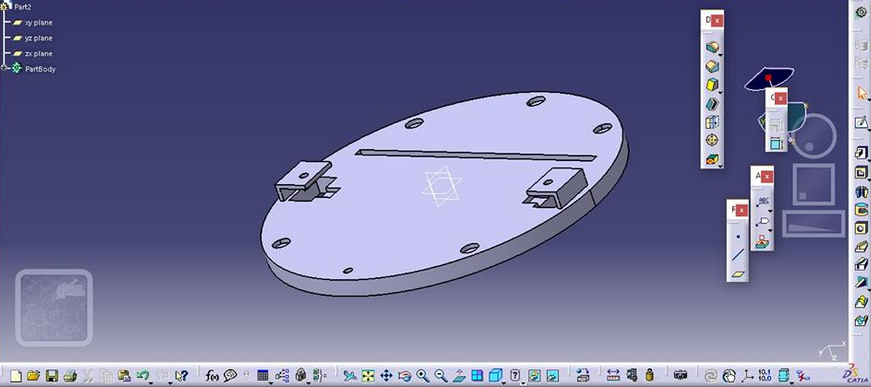
\includegraphics[scale=0.5]{figuras/estrutura_circular.png}
				\caption{Estrutura circular de integração dos subsistemas.}
				\label{img:estrutura_circular}
			\end{figure}

			\begin{table}[H]
				\centering
				\caption{Especificações roda tracionada}
				\label{tab:especificacoes_roda}
				\begin{tabular}{|c|c|}
					\hline
					\multicolumn{2}{|c|}{\cellcolor[HTML]{C0C0C0}\textbf{Especificação da Roda}}                 \\ \hline
					\textit{\textbf{Material}}                             & Roda plástica com pneu de borracha. \\ \hline
					\textit{\textbf{Diâmetro externo}}                     & 65 mm                               \\ \hline
					\textit{\textbf{Largura pneu}}                         & 26 mm                               \\ \hline
					\textit{\textbf{Diâmetro interno para engate do eixo}} & 5,4 mm "I"                          \\ \hline
				\end{tabular}
			\end{table}

			A parte superior da estrutura, ou seja, a tampa, será fabricada em PVC ou em acrílico. A escolha de um material plástico deve-se a facilidade de manuseio, facilitando molda-lo à forma desejada. Deixa a estrutura mais leve, fazendo com que o motor realize menos trabalho, e pode suportar valores altos de cargas, resistindo a impactos. O material acrílico (METACRILATO DE METILA) possui (densidade relativa de 1.19 g/cm3), resistente a água e boa resistência segundo a Figura \ref{img:acrilico}:
			ARRUMAR TABELA!!!!!
			\begin{figure}[H]
				\centering
				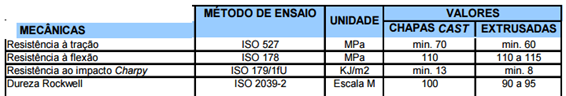
\includegraphics[scale=0.8]{figuras/tabela_acrilico.png}
				\caption[Valores de propriedades mecânicas do Acrílico]{Valores de propriedades mecânicas do Acrílico. Adaptado de \href{http://www.indac.org.br/arquivos/acrilico\_indac.pdf}{Indac}.}
				\label{img:acrilico}
			\end{figure}

			Na tabela \ref{tab:pvc} são apresentados os valores referentes ao PVC.

			\begin{table}[H]
				\centering
				\caption{Valores das propriedades mecânicas do PVC.}
				\label{tab:pvc}
				\begin{tabular}{|c|c|c|c|}
					\hline
					\textit{\textbf{Materiais}} & \textit{\textbf{\begin{tabular}[c]{@{}c@{}}Resistência a tração\\ (N/mm\textsuperscript{2})\end{tabular}}} & \textit{\textbf{\begin{tabular}[c]{@{}c@{}}Módulo de elasticidade\\ (kN/mm\textsuperscript{2})\end{tabular}}} & \textit{\textbf{\begin{tabular}[c]{@{}c@{}}Densidade\\ (kg/m\textsuperscript{3})\end{tabular}}} \\ \hline
					PVC                         & 55                                                                                       & 3.5                                                                                         & 1400                                                                          \\ \hline
				\end{tabular}
			\end{table}

			Ambos os materiais apresentam boa resistência à tração e podem ser aplicados ao projeto e irão proteger os circuitos, baterias, motores e outros equipamentos sensíveis em seu interior. A placa de acrílico ou de PVC cortado e usinado para se encaixar na estrutura montada utilizando parafusos e porcas. Os parafusos irão facilitar o trabalho de encaixe e desencaixe da tampa de acrílico para ajustes e limpezas das peças, além de fixar melhor. Se a tampa fosse colada na estrutura não haveria essa possibilidade.

	% subsection solução_1 (end)
% section alimentação (end)

\section{Estrutura da Base de Recarga} % (fold)
\label{sec:estrutura_da_base}
	
	O robô terá uma base de recarga automática responsável pelo guiamento do sistema pelo ambiente, pelo recarregamento da bateria e por abrigar e alimentar o Raspberry Pi que fará os cálculos de movimento do sistema.

	\subsection{Solução} % (fold)
	\label{sub:solução}
		
		O requisito é que o robô ao identificar que está com bateria baixa irá seguir para a base seguindo o sinal emitido por ela. A estrutura da base não necessita ter grande porte, por ser fixa e possuir menos equipamentos em seu interior. A base terá uma carcaça quadrada de dimensões 250x250x200mm, como se fosse uma caixa e assim como o robô aspirador, será feito em acrílico ou PVC pela leveza, resistência e custo. Como é uma peça de plástico também evitará condução de corrente, mantendo a proteção do usuário contra choques.  O conector será do tipo magnético, pois no momento em que for ocorrer o encaixe entre as peças do conector, esta possa ser feita de modo mais certeiro e ficará na face oposta à que fica apoiada na parede.

		\begin{figure}[H]
			\centering
			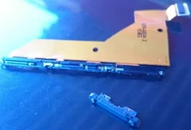
\includegraphics[scale=0.8]{figuras/conector_mag.png}
			\caption{Conectores magnético modelo Sony Xperia.}
			\label{img:conectores}
		\end{figure}

		\begin{figure}[H]
			\centering
			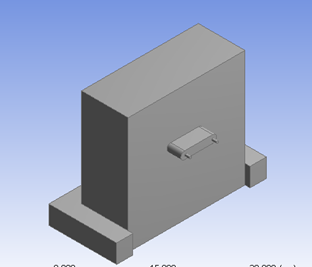
\includegraphics[scale=0.8]{figuras/estrutura_base.png}
			\caption{Estrutura da base de recarga.}
			\label{img:estrutura_base}
		\end{figure}	
	

	% subsection solução (end)
% section estrutura_da_base (end)

\section{Sucção} % (fold)
\label{sub:aspirador}
	
	Dentro dos principais objetivos, é necessário construir de forma objetiva um aspirador de pó. Deve-se projetar um sistema de sucção eficiente para que sugue desde de partículas de poeiras a resto de alimentos, estudo da dinâmica do processo, ou seja, o fluxo de ar dentro do motor do aspirador. Há dois tipos principais de modelos para ser utilizado em aspiradores de pó, um é o mais clássico utilizando ventiladores controlados por motores elétricos fazendo com que a pressão no interior do motor seja menor que a do ambiente e a diferença de pressão força o ar a entrar no aspirador seguindo até encontrar uma saída. Um filtro é colocado antes do ventilador para que seja separado a poeira do ar. O outro tipo é chamado de ciclone e não necessita de um filtro, pois pelo mesmo princípio da diferença de pressão o ar é sugado mas segue em uma trajetória helicoidal em torno de um cone e por efeito de força centrípeta a poeira é jogada para as paredes do aspirador e depois se depositam do inferior do aspirador onde são removidas, enquanto o ar percorre na direção contrária.

	\subsection{Solução} % (fold)
	\label{sub:solução}
		
		Para o projeto foi escolhido o primeiro modelo do ventilador com filtro, pois  é uma solução com um custo menor e de fácil implementação se comparado ao sistema ciclone. Serão integradas nesse sistema escovas abaixo da linha de sucção, conhecidas como vassouras mágicas, que irão facilitar o transporte e direcionar a poeira para dentro do aspirador. Serão escolhidos dois coolers comerciais com uma vazão de ar por volta de 160 m\textsuperscript{3}/h, que serão colocados lado a lado dentro de um sistema hermeticamente fechado.

		A geometria do sistema busca diminuir a área de escoamento para aumentar a velocidade do fluído na ponta de sucção, utilizando do principio de conservação do fluxo de massa do sistema. O sistema de vedação será construído utilizando acrílico colado e mangueiras sanfonadas. Também será utilizado um motor para o acionamento da escova. Para o armazenamento do pó, será projetada uma caixa retangular de plástico com tampa. No momento da limpeza do depositório, o proprietário do aspirado deve apenas desencaixar a parte móvel, retirar as impurezas e encaixar novamente na tampa.

		O dispositivo de sucção da poeira está baseado na predição fornecida pela Equação da Continuidade. A equação descreve que o fluxo de massa que entra no sistema e o que sai no sistema é igual, de forma que a diminuição da seção transversal da tubulação causa um aumento da velocidade do escoamento, que por usa vez vai ter uma capacidade maior de arrastar partículas para dentro do sistema. Por sua vez, uma velocidade maior em um escoamento causa uma diminuição da pressão pelo princípio de Bernoulli e essa variação da pressão causa uma força que auxilia a aspiração de partículas.

		Os dados relativos ao fluxo de massa e potência dos coolers comerciais é muito limitado. Assim o dimensionamento do sistema será realizado utilizando uma simulação de base no Ansys em conjunto com experimentos empíricos em protótipos simplificados. Para primeira análise, foi realizada uma simulação com as condições de contorno definidas pelo fluxo de massa constante na entrada e na saída, com um valor de 0,026Kg/s ou  cerca de 50 CFM. A simulação mostrou uma velocidade de saída do escoamento de 5 m/s e a velocidade de entrada do ar de 19 m/s.

		\begin{figure}[H]
			\centering
			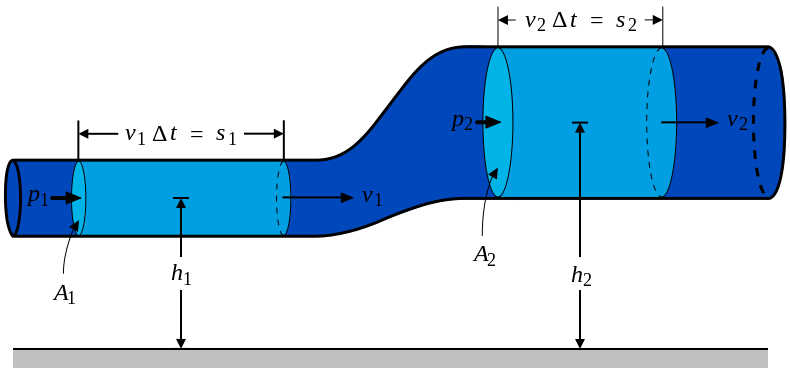
\includegraphics[scale=0.4]{figuras/succao.png}
			\caption{Demonstração da equação da continuidade, equação que descreve a conservação de massa do escoamento.}
			\label{img:succao}
		\end{figure}

		\begin{equation}\label{1}
		\frac{v^{2}}{2} + gh + \frac{p}{\rho} = constante
		\end{equation}
		
		ou
		
		\begin{equation}
		\frac{\rho v^{2}}{2} + \rho gh + p = constante
		\end{equation}

		$v$ = velocidade do fluido ao longo do condutor

		$g$ = aceleração da gravidade
		
		$h$ = altura em relação a um referencial
		
		$p$ = pressão ao longo do recipiente
		
		$\rho$ = massa específica do fluido

		Segue a equação da continuidade na sua forma de integral:

		\begin{equation}
		\frac{dq}{dt} + \iint_{s}^{ }j . dS= \sum
		\end{equation}
		
		onde $S$ é qualquer superficie fechada imaginária, com um volume V;

		$\iint_{s}^{ }dS$ se refere a integral de superficie sobre a superficie fechada

		$q$ é o amontoado total do volume

		$j$ é o fluxo de q

		$t$ é o tempo


		A analise do fluxo de massa realizada no software \textit{Ansys} está apresentada na Figura \ref{img:analise_fluxo}.

		\begin{figure}[H]
			\centering
			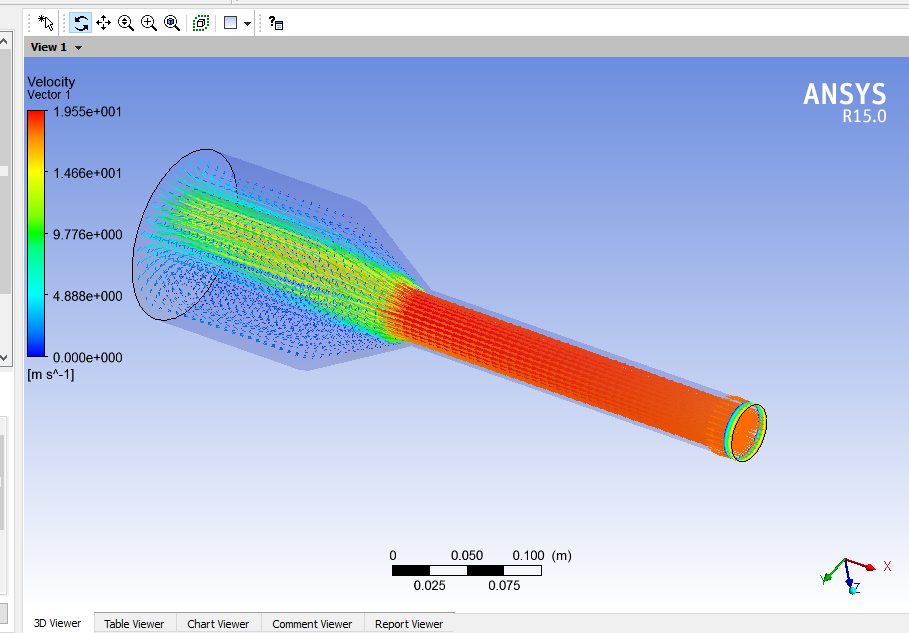
\includegraphics[scale=0.4]{figuras/analise_fluxo.png}
			\caption{Simulação do Ansys com o fluxo de massa de um cooler comercial.}
			\label{img:analise_fluxo}
		\end{figure}



	% subsection solução (end)
% section aspirador (end)

\section{Sensoriamento} % (fold)
\label{sec:sensoriamento}
\subsection{Contextualização}

Diante do projeto proposto, a equipe de eletrônica a princípio se propõe a desenvolver parte da automação e do controle do aspirador de pó, para isso o projeto eletrônico foi dividido em 3 partes, sendo elas:
  \begin{itemize}
    \item Instrumentação.
    \item Comunicação.
    \item Controle.
  \end{itemize}
% section contextualização (end)

\subsection{Instrumentação} % (fold)
\label{sub:instrumentação}

% subsection instrumentação (end)

A parte de instrumentação tem como principal objetivo solucionar o problema de colisão indesejada com a parede e outros móveis presentes na casa, para isso se faz necessário o uso de alguns componentes relativamente simples porem com grande aplicação, são eles:
 
  \subsubsection{Sensor de distância por infravermelho} 
  \label{sub:Sensor_de_distância_por_infravermelho}
    É possível utilizar um par formado por um LED emissor e um receptor de infravermelho para a detecção de obstáculos em robótica, como descrito por Lee e Chong (2011).  Essa solução será adotada no presente projeto para a detecção de objetos no trajeto do robô e segurança do protótipo \cite{detectar_objeto}.

    A solução foi escolhida devido a facilidade de obtenção dos componentes e baixo custo além da possibilidade de projetar o sensor ao invés de realizar a compra do módulo pronto, diminuindo mais ainda os custos de produção do robô aspirador.

    O circuito da figura abaixo serve para validar o sistema de detecção de obstáculos.

    \begin{figure}[H]                                       
      \centering                                            
      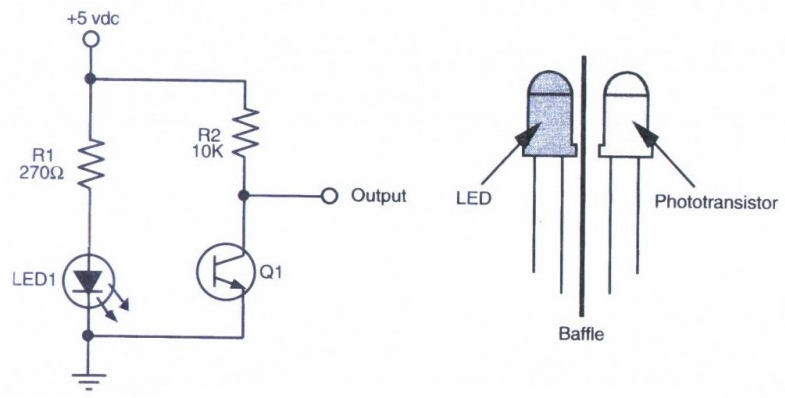
\includegraphics[scale=0.3]{figuras/sensor_proximidade.png} 
      \caption{Circuito de um sensor de proximidade usando LED emissor de infravermelho e um fototransistor.}    
      \label{img:sensor_proximidade}                                
    \end{figure}                                            

    A luz infravermelha gerada pelo LED emissor é refletida pelo objeto onde ela incide e atinge o fototransistor receptor que entra na sua zona de condução. Dependendo da quantidade de luz refletida de volta para o fototransistor, ele detecta o objeto a frente. 

    \begin{figure}[H]                                                           
      \centering                                                                
      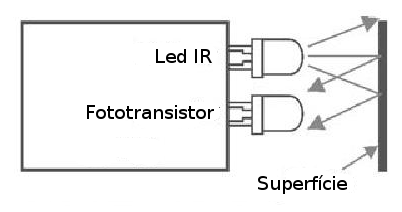
\includegraphics[scale=0.5]{figuras/funcionamento_sensor_obstaculo.png}               
      \caption{ Esquema de funcionamento do sensor de obstáculos por IR (infravermelho).}    
      \label{img:esquema_sensor_proximidade}                                            
    \end{figure}         

    Através do circuito então, quando um objeto se aproximar do sensor, a uma distância mínima que será especificada, um sinal será emitido para o controlador que irá acionará os motores para desviarem do obstáculo, para garantir a eficiência dessa solução serão utilizados no mínimo 5 sensores, 3 na parte inferior de forma a analisar a frente e as laterais do robô, um na parte superior para detectar a proximidade de obstáculos altos como mesas, e um abaixo do aspirador para indicar um possível desnivelamento a fim de evitar uma queda do mesmo.
                               
  \subsubsection{Demultiplexador}                        
  \label{sub:demultiplexador}
    Visto que a quantidade de pares IR presente no projeto é maior que 5 se faz necessário o uso de uma estratégia de alimentação para não sobrecarregar o microprocessador. Optou-se então por utilizar um demultiplexador possibilitando assim o chaveamento dos emissores de IR através do clock do microprocessador.

    O componente escolhido para esse projeto foi o 4051, circuito integrado CMOS, consiste num Multiplexador/Demultiplexador de 8 canais que pode trabalhar tanto com sinais analógicos como digitais.\cite{newtoncbraga}

  \begin{figure}[H]                                                           
    \centering                                                                
    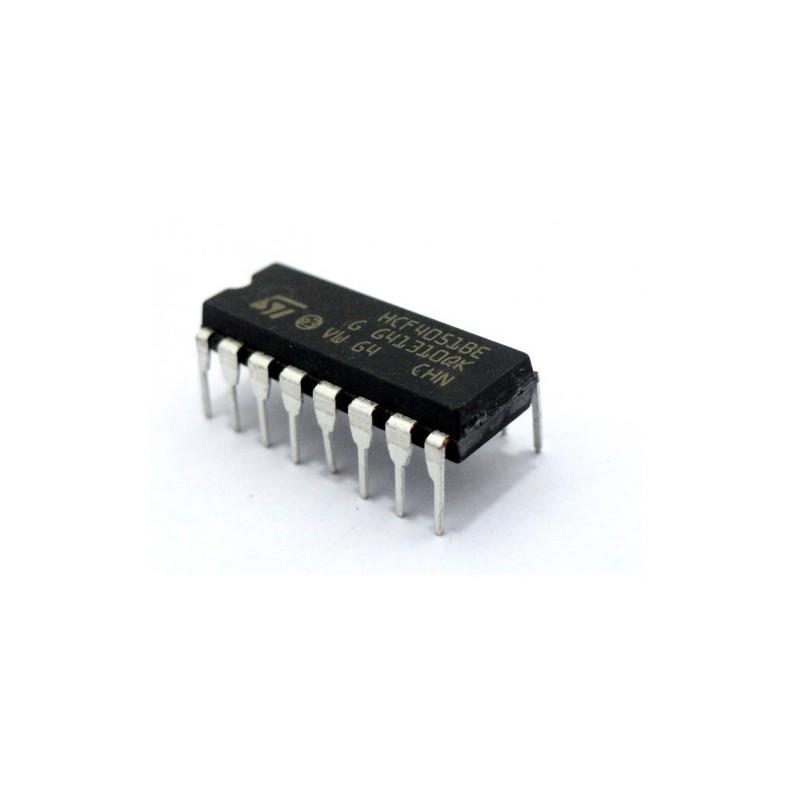
\includegraphics[scale=0.2]{figuras/multiplexador.png}             
    \caption{ CI CMOS 4051 multiplexador/demultiplexador de 8 canais.} 
    \label{img:multiplexador}                                            
  \end{figure}                                                                

  \subsubsection{Medidor de Bateria}
  \label{sub:Medidor_de_bateria}
    O aspirador de pó não pode ficar sem bateria no meio da execução da limpeza. Para conferir o nível de bateria, será utilizado um comparador de tensão. De forma que, assim que o medidor verificar que o nível da bateria está ficando muito reduzido, um sinal será enviado ao microprocessador que irá interromper o ciclo de limpeza e enviar o robô para a base de carregamento.

    Escolheu-se um circuito comparador que irá comparar a tensão da bateria com até 10 níveis de referência determinados de acordo com a tensão máxima da bateria e o mínimo aceitável para que o robô retorne à base. Essa comparação irá ocorrer por meio de amplificadores operacionais (Amp Op) que irão comparar a tensão que está vindo da bateria com aos níveis de referência. A saída do Amp Op será 1 se o sinal da bateria for maior do que a referência daquele amplificador ou será 0 se o sinal da bateria for menor do que a referência. Para tornar visível o nível da bateria, na saída de cada comparador será adicionado um LED.

    Além de acender ou não os LEDs, cada saída do comparador vai enviar um sinal para o controlador informando o nível da bateria para que ele possa interromper o ciclo de limpeza e enviar o robô para base.

% section instrumentação (end)

\subsection{Hardware para Comunicação}
\label{sub:Hardwar_para_Comunicação}
  A parte de comunicação tem como objetivo coletar informações vindas dos sensores já apresentados, interpreta-las e envia-las para a base onde é feito o intefaceamento com o usuário através de um aplicativo para celular, para essa comunicação serão utilizados 2 microprocessadores, são eles:

    \subsubsection{Arduíno}
    Para controlar corretamente as informações obtidas por todos os sensores da parte de instrumentação do projeto é necessário um processador com uma grande quantidade de portas analógicas e digitais, sendo assim utilizaremos o Arduíno Mega, que possui as seguintes características:

    \begin{figure}[H]                                                  
      \centering                                                       
      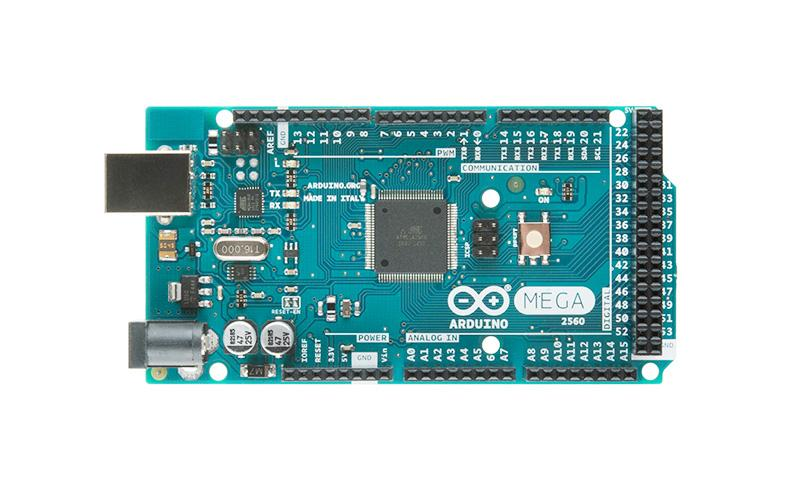
\includegraphics[scale=0.4]{figuras/arduino_mega.png} 
      \caption{Arduíno Mega.}                  
      \label{img:arduino_mega}                                             
    \end{figure}                                                       

    \begin{itemize}
      \item Microcontrolador: ATmega2560
      \item Voltagem de Alimentação: 5V
      \item Voltagem de entrada (recomendada): 7-12V
      \item Voltagem de entrada (limites): 6-20V
      \item Pinos digitais I/O: 54 (dos quais 14 podem ser saídas PWM)
      \item Pinos de entrada analógica: 16
      \item Corrente contínua por pino I/O: 40 mA
      \item Corrente contínua para o pino 3.3V: 50 mA
      \item Memória flash: 256 KB com 4 KB usado para bootloader
      \item SRAM: 8 KB
      \item EEPROM: 4 KB
      \item Velocidade de Clock: 16Mhz
    \end{itemize}
  
  \subsubsection{Módulo de WiFi}
  \label{sub:Modulo_de_wifi}
    Para que o Arduíno possa enviar as informações coletadas para a base é necessário que o mesmo se conecte a rede sem fio, para isso utilizaremos o módulo WiFi ESP8266 ilustrado na figura abaixo.

  \begin{figure}[H]                                      
    \centering                                           
    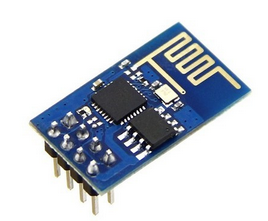
\includegraphics[scale=0.8]{figuras/modulo_wifi.png}
    \caption{Módulo WiFi ESP8266}                              
    \label{img:modulo_wifi}                             
  \end{figure}                                           

  \subsubsection{Raspberry Pi}
  \label{sub:Raspberry}
    Na base para o tráfego de dados, a placa escolhida foi a Raspberry Pi 2 modelo B, este modelo apresenta:

  \begin{figure}[H]                                      
    \centering                                           
    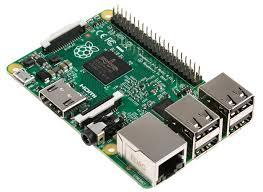
\includegraphics[scale=0.8]{figuras/rasp.jpg} 
    \caption{Raspberry Pi 2 B.}                        
    \label{img:Rasp}                              
  \end{figure}                                           

  \textbf{Especificações:}
  \begin{itemize}                                                     
    \item Chip: Broadcom BCM2836 SoC
    \item Arquitetura: Quad-core ARM Cortex-7
    \item CPU: 900Mhz
    \item Memória RAM: 1GB
    \item GPU Broadcom VideoCore IV
    \item Tensão de operação: Micro USB socket 5V/2ª
    \item Dimensões: 85 x 56 x 17 mm
 \end{itemize}                                                       
  
  \textbf{Conectores:}
  \begin{itemize}                                                     
    \item 4 portas USB
    \item GPIO de 40 pinos
    \item Full HDMI
    \item Ethernet 10/100 (RJ45)
    \item Saída de vídeo via HDMI, Composite (PAL e NTSC) ou Raw LCD (DSI)
    \item Saída de áudio via conector de 3,5mm
    \item Camera interface (CSI)
    \item Slot MicroSD
    \item VideoCore IV 3D graphics core
  \end{itemize}

  Com esse modelo, é possível realizar conexões com a internet e enviar informações ao usuário ou a um banco de dados, por exemplo.

\subsection{Controle} % (fold)
	\label{sub:controle}

	\subsubsection{Formas de controle de Sistemas}

		“Um sistema de controle é um conjunto de componentes organizados de forma a conseguir uma resposta desejada de um sistema”, \cite{mello}. Para cada função de uma máquina que se deseja controlar deve haver um sistema de controle especifico. Existem dois tipos de controle: o de malha aberta e o de malha fechada, e um sistema de controle é dividido em subsistemas e agrupamentos de processos, a fim de se obter saídas por meio do desempenho desejado de acordo com a entrada utilizada especificamente \cite{mello}.

		\begin{figure}[H]
			\centering
			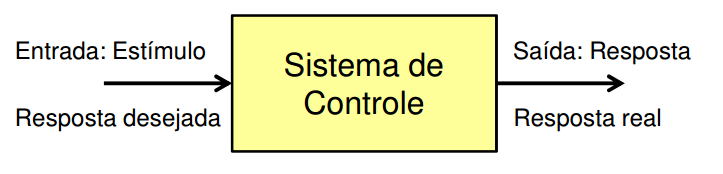
\includegraphics[scale=0.5]{figuras/sistema_controle.png}
			\caption{Sistema de controle representado em blocos. Fonte \cite{mello}.}
			\label{img:sistema_controle}
		\end{figure}

		Para o desenvolvimento de um sistema de controle são necessários alguns elementos básicos, demonstrados na figura abaixo, são eles:

		\begin{itemize}
			\item Planta: Objeto real a ser controlado.
			\item Variável de controle: saída do sistema.
			\item Valor esperado: valor desejado da variável de controle baseados nos requisitos do sistema.
			\item Controlador: Agente que calcula o sinal de controle necessário.
			\item Atuador: dispositivo que transforma energia em algum tipo de movimento.
			\item Sensor: dispositivo que converte um elemento físico em um sinal.
			\item Distúrbio: Fator inesperado.
		\end{itemize}

		\begin{figure}[H]
			\centering
			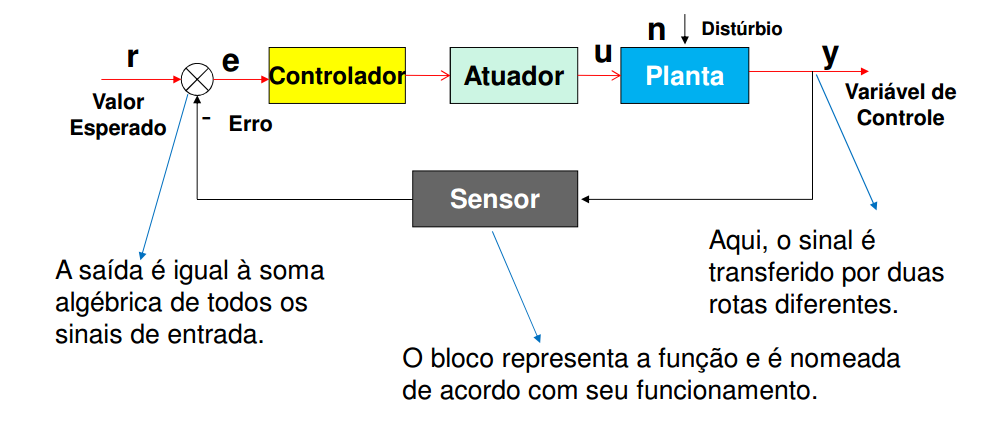
\includegraphics[scale=0.4]{figuras/diagrama_blocos_controle.png}
			\caption{Diagrama de blocos de um sistema de controle. Fonte \cite{mello}.}
			\label{img:diagrama_sistema_controle}
		\end{figure}

		No controle de malha aberta (Open Loop Systems), não há realimentação, somente um sinal de controle na entrada e é esperado que na saída à variável controlada consiga atingir um determinado valorou comportamento desejado. Nesse tipo de sistema não é observada evolução do processo para determinação do sinal de controle. A entrada não depende da saída, então um dos problema desse tipo de sistema é que só é possível ter a saída esperada se não ocorrer perturbações internas e externas, por que o controlador continuará funcionando normalmente, como se não tivesse ocorrido qualquer perturbação e a resposta não terá valor para as novas características do sistema \cite{silva}. As principais vantagens de se utilizar esse sistema de controle é o custo e a simplicidade.

		Já no controlador de malha fechada (Closed Loop Systems), o sistema tem controle retroativo, realimentado, onde necessita de informações da saída do controle por meio de sensores ou transdutores que compara o sinal de saída com uma referência e corrige a saída caso ela esteja desviada dos parâmetros programados \cite{silva}. As principais vantagens em se utilizar esse sistema de controle são a rejeição a perturbações, atenuação de ruídos, melhor controle do estado transitório, menor sensibilidade a mudança de parâmetros, entre outros. A principal desvantagem é o aumento da complexidade e custo do sistema.

		\subsubsubsection{Sistema de Controle do R2-PI2}

			A parte de controle tem como objetivo desenvolver um sistema capaz de monitorar e controlar a movimentação do aspirador para garantir que os motores sejam devidamente alimentados e juntamente com a parte de instrumentação e comunicação possa garantir a locomoção do robô durante a limpeza sem riscos de colisão com obstáculos.

			O controlador por ora escolhido, Arduino, irá controlar o funcionamento dos motores carrinho e dos sensores. Abaixo encontra-se o diagrama de blocos para o sistema em malha fechada do controle do R2-P12.

			\begin{figure}[H]
				\centering
				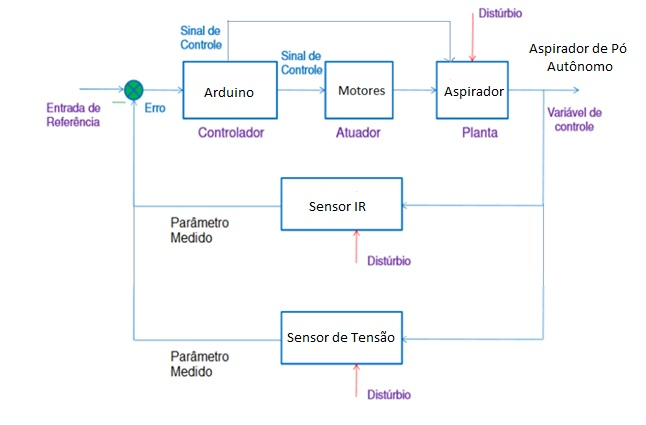
\includegraphics[scale=0.55]{figuras/diagrama_blocos_R2PI2.png}
				\caption{Diagrama de blocos do sistema de controle do R2-PI2. Fonte \cite{mello}.}
				\label{img:diagrama_sistema_controle}
			\end{figure}

			Como mostrado no diagrama, o controlador irá enviar sinais para os motores permitindo que eles sejam ligados ou desligados, fazendo o carrinho se movimentar de acordo com os parâmetros medidos pelos sensores infravermelhos (IR). 

			Serão utilizados sensores IR configurados como detectores de proximidade, na parte frontal  e lateral do aspirador, evitando possíveis colisões com obstáculos em seu caminho, e embaixo dele para evitar vãos como escadas e impedir a queda do robô. Encoderes serão utilizados como controle de posição e também no auxílio da movimentação das rodas quando o aspirador girar para desviar de obstáculos. O monitoramento será contínuo, portanto sempre que houver algum obstáculo ao alcance dos sensores , o controlador enviará um sinal para os motores, impedindo que ocorra choques com objetos no caminho. 

			Será monitorado também, o nível de bateria do robô, quando ele estiver abaixo de um limite que será estabelecido, o controlador enviará um sinal para que o robô possa então retornar para a base e carregar sua bateria. Os componentes envolvidos nessa área são apresentados a seguir.

			\begin{enumerate}
				\item \textbf{Ponte H}:

					Para que se possa controlar a direção e a velocidade dos motores , é necessário que a corrente elétrica possa fluir nas duas direções dentro de sua bobina, gerando campos magnéticos com intensidade e sentidos opostos. A configuração mais utilizada para controlar a corrente nesse projeto é um driver em ponte H (INOUE e OSUKA, 2004).

					O circuito da Ponte H é constituído por quatro transistores que atuam como chave e que, dependendo da configuração do chaveamento, determinam o sentido de rotação dos motores, como pode ser observado na Figura \ref{img:configH}.

					\begin{figure}[H]
						\centering
						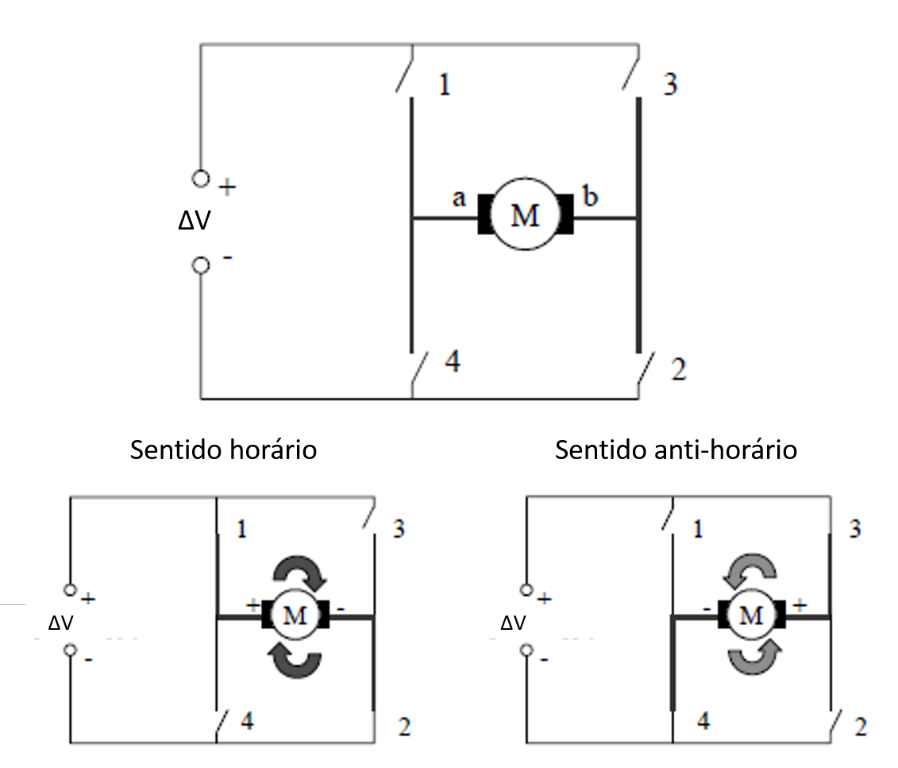
\includegraphics[scale=0.3]{figuras/configH.png}
						\caption{Configurações da Ponte H.}
						\label{img:configH}
					\end{figure}

					A princípio a ponte H escolhida segue o modelo apresentado na Figura \ref{img:modeloH}. 

					\begin{figure}[H]
						\centering
						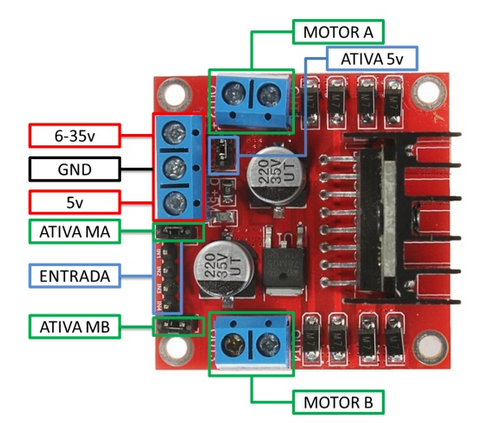
\includegraphics[scale=0.6]{figuras/modeloH.png}
						\caption{Ponte H.}
						\label{img:modeloH}
					\end{figure}

					A escolha foi feita baseando-se na compatibilidade do drive com os motores que devem ser utilizados na movimentação do aspirador.
				\item \textbf{PWM}:

					O controle das velocidades dos motores será feito por meio de chaveamento em frequência constante, gerado pelas saídas digitais do controlador. Para isso utiliza-se o conceito de Pulse-Width Modulation (Modulação por largura de pulso), ou PWM. Com uma onda quadrada com frequência constante e razão cíclica (duty cycle) ajustável , é possível transferir uma determinada quantidade de potência desejável através do valor médio de tensão do sinal \cite{ahmedi}.

					Segundo \cite{ahmedi}, a tensão média de saída é dada por

					\begin{equation}\label{3}
						V_{0} = \frac{Ton.vi}{T}
					\end{equation}
					Onde  é a tensão média de saída,  é o período em segundos em que o sinal fica em nível alto, T o período total do sinal e Vi a tensão de nível alto.

					A potência de saída do sinal pode ser descrita como:

					\begin{equation}
					P = V_{0} . I_{0}
					\end{equation}

					Sendo P a potência de saída,  a tensão de saída e  a corrente de saída. Portanto a partir das equações anteriores pode-se afirmar que:

					\begin{equation}
					V_{0} = Vi . d
					\end{equation}

					onde:

					$d = \frac{Ton}{T}$

					sendo  o duty cycle. A partir da lei de Ohm tem-se então que :

					\begin{equation}
					I_{0} = \frac{d . Vi}{R}
					\end{equation}

					E a potência de saída é dada por:

					\begin{equation}
					P_{0} = \frac{(D . Vi)^{2}}{R}
					\end{equation}

					Considerando-se uma carga totalmente resistiva, pode-se controlar a potência entregue de maneira proporcional a largura de pulso ao quadrado.

					Deve-se observar a frequência de trabalho, para não ultrapassar os limites do hardware de potência em casos onde há carga indutivas, como motores, é necessário pulsar uma frequência que faça a corrente estável para uma mesma largura de pulso, suavizando assim o movimento do motor.

				\item \textbf{Encoder}:

					Os encoders são sensores acoplados no motor para medir a velocidade e posição angular de acordo com a rotação sensoriada por ele. A especificação dos encoders absolutos são medidas em contagem por rotação, CPR, pois de acordo com o número de divisões do encoder e o tamanho da roda conhecem as velocidades, angular e linear, e também a trajetória percorrida \cite{braga}.

					\begin{figure}[H]
						\centering
						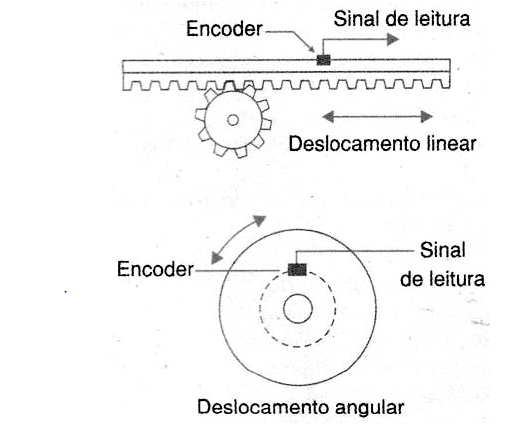
\includegraphics[scale=0.6]{figuras/encoder.png}
						\caption{Sistema de funcionamento de um encoder absoluto.}
						\label{img:encoder}
					\end{figure}

					A posição relativa do aspirador de pó é uma variável muito importante para a navegação e localização que pode ser medida através do uso de encoders [3]. Fixado junto ao motor, o encoder rotacional irá medir a quantidade de rotações do motor e, portanto, possibilitar a obtenção de informações sobre a velocidade angular e posição relativa. 

					Para esse projeto escolheu-se o módulo encoder P17 \ref{img:modulo_encoder} que realiza a leitura do sentido do giro e pode ser integrado ao Arduíno.

					\begin{figure}[H]
						\centering
						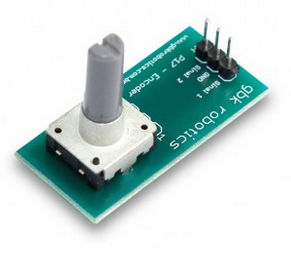
\includegraphics[scale=0.6]{figuras/modulo_encoder.png}
						\caption{Módulo encoder.}
						\label{img:modulo_encoder}
					\end{figure}

			\end{enumerate}



	% subsection controle (end)
% section instrumentação (end)


\section{Comunicação} % (fold)
\label{sub:comunicação}
	De acordo com o apresentado nesta documentação de projeto, a solução proposta envolve diversos módulos funcionais, como o robô em si, a base fixa, e o sistema de controle. A partir de uma visão de alto nível do projeto, como a apresentada na Figura \ref{img:arq_comu}, é possível observar de maneira clara os módulos que deverão se comunicar para garantir o funcionamento do sistema como um todo.

	\begin{figure}[H]
		\centering
		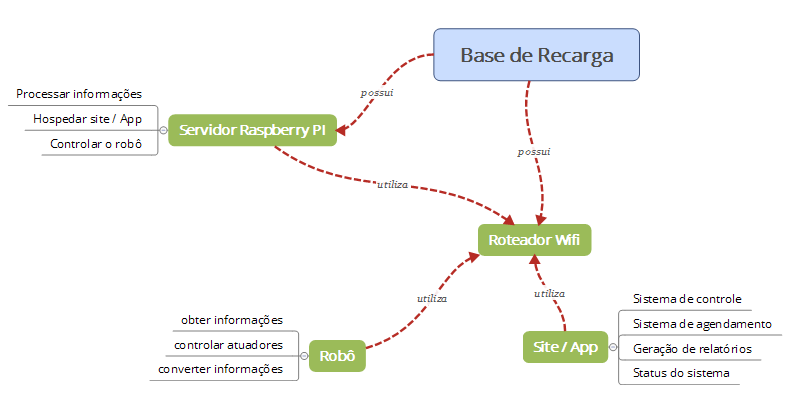
\includegraphics[scale=0.8]{figuras/arquitetura_comunicacao.png}
		\caption{Arquitetura de comunicação do sistema}
		\label{img:arq_comu}
	\end{figure}

	Com o objetivo de garantir que a solução seja confiável e resistente a situações críticas, como a falta de internet, por exemplo, o sistema foi planejado para disponibilizar uma sub-rede interna, tendo como fonte a base de recarga do robô. Cada módulo que necessita de comunicação deverá se conectar a rede, viabilizando o funcionamento do sistema mesmo em momentos com falha de internet, já que todos os envolvidos compartilham o mesmo ambiente.

	A comunicação entre o robô (\textit{arduino}) e a base (raspberry) fará uso desta rede wifi, a partir da utilização de um módulo wifi, o \textit{arduino} poderá acessar a rede, possibilitando a comunicação via tcp/ip. Já a \textit{raspberry} se conectará a rede via cabo \textit{ethernet}.

	O roteador utilizado é da familia D-link, seguindo o protocolo de certificação WPA2, que utiliza o EAS (Advanced Encryption Standard), como sistema de encriptação. Segundo \cite{wpa2}, este protocolo possui uma confiabilidade bem maior que a encontrada em seu antecessor, WPA. Ainda de acordo com \cite{wpa2}, este sistema de segurança envolve um algoritmo de criptografia robusto, utilizando chaves de 128 a 256 bits maximizando a segurança da rede.


	O núcleo da rede, ou seja, o ponto central da comunicação do sistema se encontra na base de recarga do robô, que está detalhada no tópico a seguir.

	\subsection{Base de recarga}

	A base de recarga do robô sustentará todo o sistema de inteligência da solução, assim como a sub-rede que possibilitará a comunicação entre os módulos. Será utilizada uma \textit{raspberry PI} como servidor central do sistema, processando e controlando toda a solução. O servidor será implementado utilizando a tecnologia Ruby on Rails, no sistema operacional \textit{Raspbian} (Debian).

	Além da sustentação da \textit{raspberry}, é necessário sustentar um roteador D-link 524 para implementação e sustentação da rede wifi que será utilizada como meio de comunicação do sistema, e 3 (três) emissores infra-vermelho, utilizados para retorno do robô à base.
	
% section comunicação (end)

\section{Interface} % (fold)
\label{sub:interface}
  A interface de usuário é onde ocorre a interação entre humanos e máquinas, o objetivo desta interação é a operação e controle efetivos da máquina pelo usuário e o feedback desta, que auxilia o operador na tomada de decisões operacionais.

  Tendo em vista isso o aspirador terá uma plataforma web que contará com uma interface amigável e intuitiva facilitando o acesso à diferentes dados e funções. Essa plataforma será responsiva, isto é, se adaptará automaticamente à largura de tela do dispositivo no qual ele estará sendo visualizado. Assim o sistema se comportará como ponte entre o usuário e o aspirador.

{Para essa primeira entrega foi construído um protótipo de médica fidelidade com a ferramenta  \href{http://www.justinmind.com/}{Justmind}.} As figuras abaixo mostram os primeiros protótipos:

\begin{figure}[H]                                    
  \centering                                         
  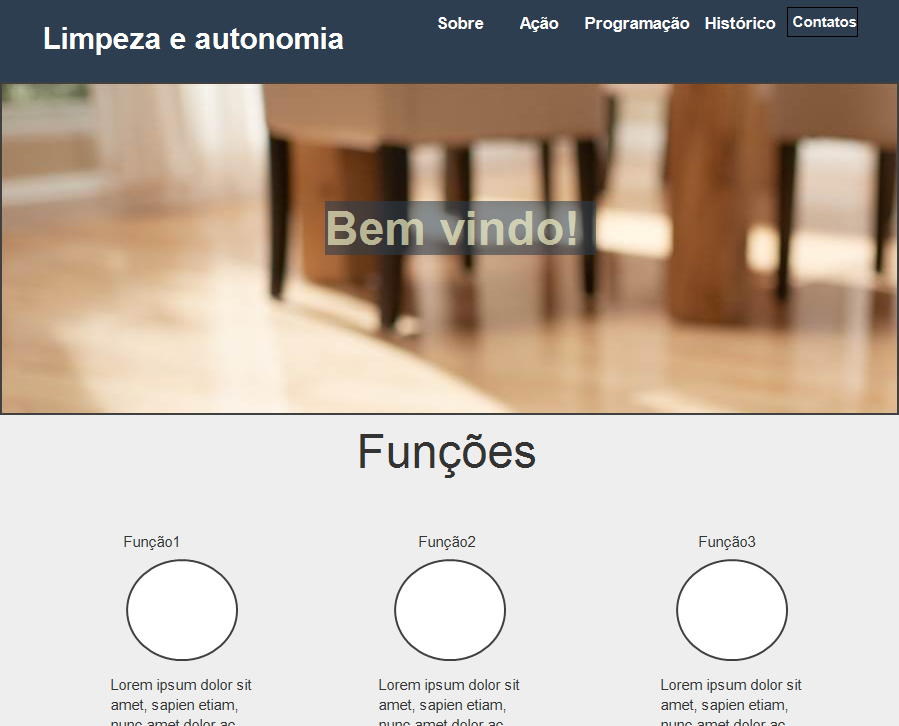
\includegraphics[scale=0.4]{figuras/home.png}
  \caption{Interfaface Home.}                        
  \label{img:inter_home}                              
\end{figure}                                         

\begin{figure}[H]                                    
  \centering                                         
  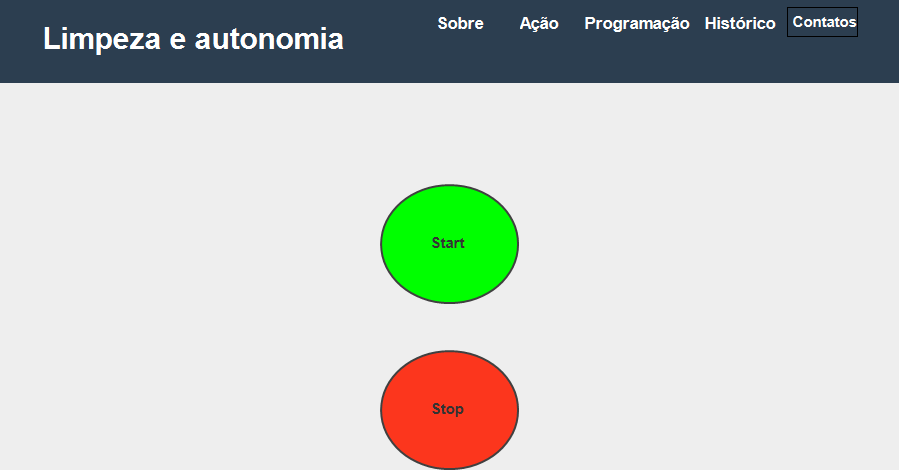
\includegraphics[scale=0.4]{figuras/comando.png}
  \caption{Interfaface Comando.}                        
  \label{img:inter_comando}                              
\end{figure}

\begin{figure}[H]                                    
  \centering                                         
  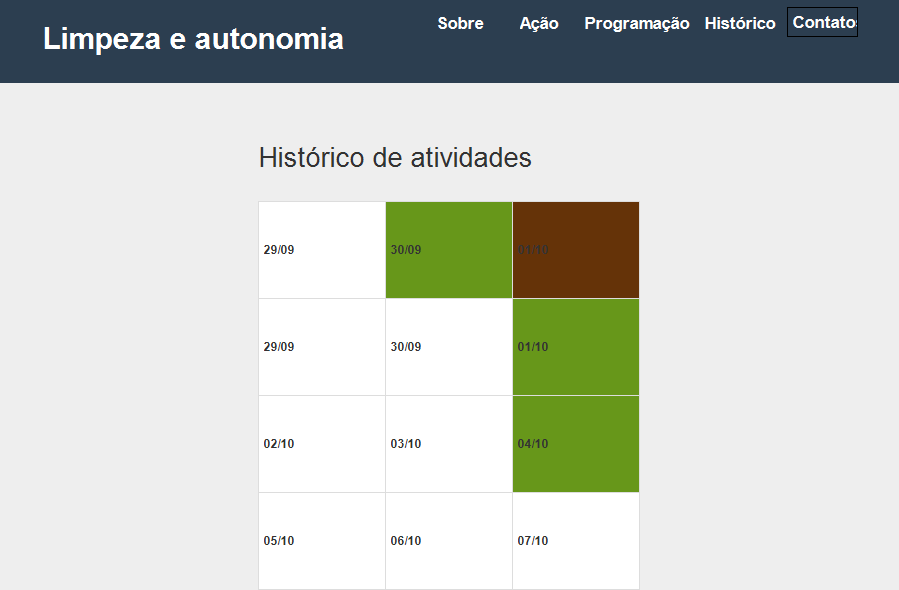
\includegraphics[scale=0.4]{figuras/historico.png}
  \caption{Interfaface Histórico.}                        
  \label{img:inter_historico}                              
\end{figure}

\begin{figure}[H]                                    
  \centering                                         
  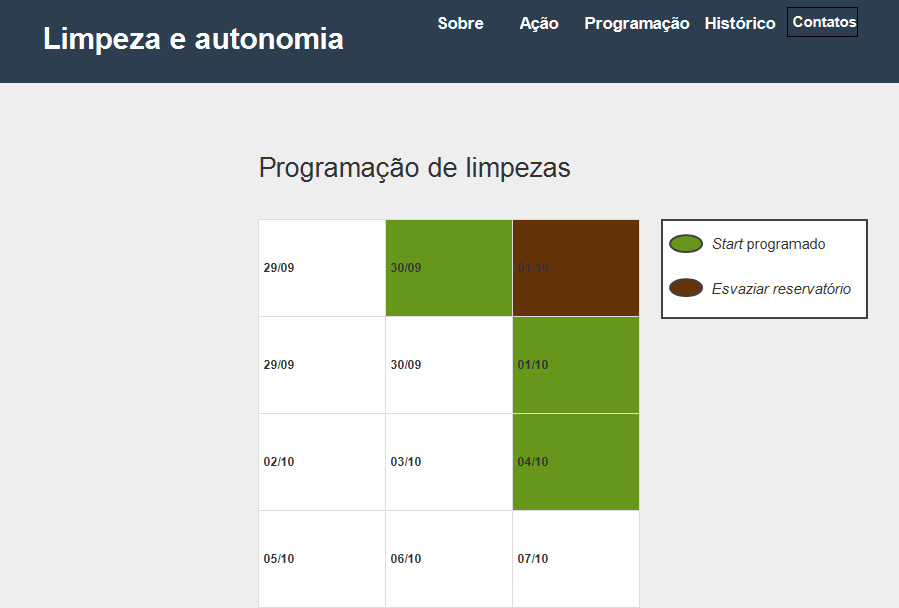
\includegraphics[scale=0.4]{figuras/programacao.png}
  \caption{Interfaface Programação.}                        
  \label{img:inter_programacao}                              
\end{figure}
% section interface (end)
